%
% Beta-Integrale
%
% (c) 2021 Prof Dr Andreas Müller, OST Ostschweizer Fachhochschule
%
\section{Die Beta-Funktion
\label{buch:rekursion:gamma:section:beta}}
Die Eulersche Integralformel für die Gamma-Funktion in
Definition~\ref{buch:rekursion:def:gamma} wurde in
Abschnitt~\ref{buch:subsection:integral-eindeutig}
mit dem Satz~\ref{buch:satz:bohr-mollerup}
von Bohr-Mollerup gerechtfertigt.
Man kann Sie aber auch als Grenzfall der Beta-Funktion verstehen,
die in diesem Abschnitt dargestellt wird.


\subsection{Beta-Integral
\label{buch:rekursion:gamma:subsection:integralbeweis}}
In diesem Abschnitt wird das Beta-Integral eingeführt, eine Funktion
von zwei Variablen, welches eine Integral-Definition mit einer
reichaltigen Menge von Rekursionsbeziehungen hat, die sich direkt auf
die Gamma-Funktion zurückführen lassen.
Daraus wird sich dann ein Beweis für die Integralformel für die
Gamma-Funktion ergeben.

\begin{definition}
\label{buch:rekursion:gamma:def:beta-funktion}
Das Beta-Integral ist das Integral
\[
B(x,y)
=
\int_0^1 t^{x-1} (1-t)^{y-1}\,dt
\]
für $\operatorname{Re}x>0$, $\operatorname{Re}y>0$.
\index{Beta-Integral}%
\end{definition}

Aus der Definition kann man sofort ablesen, dass $B(x,y)=B(y,x)$.
Für $y=1$ folgt ausserdem
\begin{equation}
B(x,1)
=
\int_0^1 t^{x-1}\,dt
=
\biggl[ \frac{t^x}{x}\biggr]_0^1
=
\frac{1}{x}.
\label{buch:rekursion:gamma:betax1}
\end{equation}
Speziell gilt $B(1,1)=1$.

\subsubsection{Rekursionsformeln für das Beta-Integral}
Aus der Definition folgt direkt
\begin{align*}
B(x,y+1)
&=
\int_0^1 t^{x-1} (1-t)^{y+1-1}\,dt
=
\int_0^1 (1-t) t^{x-1} (1-t)^{y-1}\,dt
\\
&=
\int_0^1 t^{x-1} (1-t)^{y-1}\,dt
-
\int_0^1 t^{x} (1-t)^{y-1}\,dt
\\
&=
B(x,y) - B(x+1,y)
\end{align*}
oder
\begin{equation}
B(x,y) = B(x+1,y) + B(x,y+1).
\label{buch:rekursion:gamma:betarek1}
\end{equation}
%
%XXX Vergleich mit der Rekursionsformel für Binomialkoeffizienten
%
Durch partielle Integration kann man eine weitere Rekursionsformel finden.
Dazu berechnet man
\begin{align}
B(x,y+1)
&=
\int_0^1 t^{x-1}(1-t)^{y}\,dt
\notag
\\
&=
\biggl[\frac{t^x}x(1-t)^y\biggr]_0^1
+
\frac{y}x \int_0^1 t^x(1-t)^{y-1}\,dt
\notag
\\
&=
 \frac{y}x B(x+1,y).
\label{buch:rekursion:gamma:betarek2}
\end{align}
Durch Gleichsetzen
\eqref{buch:rekursion:gamma:betarek1}
und
\eqref{buch:rekursion:gamma:betarek2}
entsteht die Rekursionsformel
\[
B(x,y)-B(x,y+1)
=
B(x+1,y)
=
\frac{x}{y}B(x,y+1)
\]
oder
\begin{equation}
B(x,y)
=
\frac{x+y}{y}B(x,y+1).
\label{buch:rekursion:gamma:betarek3}
\end{equation}

\subsubsection{Beta-Funktion und Gamma-Funktion}
Die Rekursionsbeziehung~\eqref{buch:rekursion:gamma:betarek3}
kann jetzt dazu verwendet werden, eine Darstellung der Beta-Funktion
durch die Gamma-Funktion zu finden.
Durch $n$-fache Anwendung von \eqref{buch:rekursion:gamma:betarek3}
ergibt sich zunächst
\begin{align*}
B(x,y)
&=
\frac{x+y}{y}
B(x,y+1)
=
\frac{x+y}{y}
\frac{x+y+1}{y+1}
B(x,y+2)
\\
&=
\frac{x+y}{y}
\frac{x+y+1}{y+1}
\cdot
\ldots
\cdot
\frac{x+y+n-1}{y+n-1}
B(x,y+n)
=
\frac{(x+y)_n}{(y)_n}
B(x,y+n)
\intertext{Die Beta-Funktion auf der rechten Seite kann als Integral
geschrieben werden:}
&=
\frac{(x+y)_n}{(y)_n}
\int_0^1 t^{x-1}(1-t)^{y+n-1}\,dt.
\end{align*}
Wir halten dieses Zwischenresultat für spätere Verwendung fest.

\begin{lemma}
\label{buch:rekursion:gamma:betareklemma}
Für $n\in\mathbb{N}$ gilt
\[
B(x,y+n) = \frac{(y)_n}{(x+y)_n} B(x,y).
\]
\end{lemma}

Wir streben an, mit dem Grenzübergang $n\to\infty$ aus den
Pochhammer-Symbolen Gamma-Funktionen zu machen, dazu müssen gemäss
Definition~\ref{buch:rekursion:gamma:def:definition} weitere Faktoren
$1/(n!\,n^{x-1})$ vorhanden sein.
Wir erweitern geeignet und nehmen die übrig bleibenden Faktoren in
das Integral.
So ergibt sich
\begin{align}
B(x,y)
&=
\frac{(x+y)_n}{n!\, n^{x+y-1}}
\frac{n!\,n^{y-1}}{(y)_n}
\int_0^1 n^{x} t^{x-1}(1-t)^{y+n-1}\,dt.
\notag
\intertext{Mit der Substition $s/n=t$ wird das Integral zu einem Integral
über das Interval $[0,n]$}
&=
\frac{(x+y)_n}{n!\, n^{x+y-1}}
\frac{n!\,n^{y-1}}{(y)_n}
\int_0^n
n^{x}
\biggl(\frac{s}{n}\biggr)^{x-1}
\biggl(1-\frac{s}{n}\biggr)^{y+n-1}
\,\frac{ds}{n}.
\notag
\\
&=
\frac{(x+y)_n}{n!\, n^{x+y-1}}
\frac{n!\,n^{y-1}}{(y)_n}
\int_0^n
n^{x-1}
\biggl(\frac{s}{n}\biggr)^{x-1}
\biggl(1-\frac{s}{n}\biggr)^{y+n-1}
\,ds.
\intertext{Beim Grenzübergang $n\to\infty$ wird daraus}
&=
\underbrace{\frac{(x+y)_n}{n!\, n^{x+y-1}}}_{\displaystyle \to 1/\Gamma(x+y)}
\underbrace{\frac{n!\,n^{y-1}}{(y)_n}}_{\displaystyle\to \Gamma(y)}
\int_0^n
s^{x-1}
\underbrace{\biggl(1-\frac{s}{n}\biggr)^{n}}_{\displaystyle\to e^{-s}}
\underbrace{\biggl(1-\frac{s}{n}\biggr)^{y-1}}_{\displaystyle\to 1}
\,ds.
\notag
\\
&\to \frac{\Gamma(y)}{\Gamma(x+y)} \int_0^\infty s^{x-1}e^{-s}\,ds.
\label{buch:rekursion:gamma:betagamma}
\end{align}
Das Integral im letzten Ausdruck ist die Integraldarstellung für 
die Gamma-Funktion von Definition~\ref{buch:rekursion:def:gamma},
die bis anhin noch nicht gerechtfertigt wurde.

In~\eqref{buch:rekursion:gamma:betax1} ist gezeigt worden, dass
$B(x,1)=1/x$.
Andererseits zeigt \eqref{buch:rekursion:gamma:betagamma} für $y=1$,
dass
\begin{align}
\frac1x
=
B(x,1)
&= 
\frac{\Gamma(1)}{\Gamma(x+1)}\int_0^\infty s^{x-1}e^{-s}\,ds.
\notag
\intertext{%
Wegen $\Gamma(1)=1$ und $\Gamma(x+1)=x\Gamma(x)$ finden wir nach
Multiplikation mit $x\Gamma(x)$:}
\Gamma(x)
&=
\int_0^\infty s^{x-1}e^{-s}\,ds,
\label{buch:rekursion:gamma:integralbeweis}
\end{align}
was die Integraldarstellung
von Definition~\ref{buch:rekursion:def:gamma},
der Gamma-Funktion beweist.
Durch Einsetzen der Integralformel im Ausdruck
\eqref{buch:rekursion:gamma:betagamma} folgt der folgende
Satz.

\begin{satz}
\index{Satz!Beta-Funktion und Gamma-Funktion}%
Die Beta-Funktion kann aus der Gamma-Funktion nach
\begin{equation}
B(x,y) = \frac{\Gamma(x)\Gamma(y)}{\Gamma(x+y)}
\label{buch:rekursion:gamma:betagamma}
\end{equation}
berechnet werden.
\end{satz}

%
% Info über die Beta-Verteilung
%
%
% teil1.tex -- Beispiel-File für das Paper
%
% (c) 2020 Prof Dr Andreas Müller, Hochschule Rapperswil
%
\subsection{Ordnungsstatistik und Beta-Funktion
\label{buch:rekursion:ordnung:section:ordnungsstatistik}}
\rhead{Ordnungsstatistik und Beta-Funktion}
In diesem Abschnitt ist $X$ eine Zufallsvariable mit der Verteilungsfunktion
$F_X(x)$, und $X_i$, $1\le i\le n$ sei ein Stichprobe von unabhängigen
Zufallsvariablen, die wie $X$ verteilt sind.
Ziel ist, die Verteilungsfunktion und die Wahrscheinlichkeitsdichte
des grössten, zweitgrössten, $k$-t-grössten Wertes in der Stichprobe
zu finden.
Wir schreiben $[n]=\{1,\dots,n\}$ für die Menge der natürlichen
Zahlen von zwischen $1$ und $n$.

\subsubsection{Verteilung von $\operatorname{max}(X_1,\dots,X_n)$ und
$\operatorname{min}(X_1,\dots,X_n)$
\label{buch:rekursion:ordnung:subsection:minmax}}
Die Verteilungsfunktion von $\operatorname{max}(X_1,\dots,X_n)$ hat
den Wert
\begin{align*}
F_{\operatorname{max}(X_1,\dots,X_n)}(x)
&=
P(\operatorname{max}(X_1,\dots,X_n) \le x)
\\
&=
P(X_1\le x\wedge \dots \wedge X_n\le x)
\\
&=
P(X_1\le x) \cdot \ldots \cdot P(X_n\le x)
\\
&=
P(X\le x)^n
=
F_X(x)^n.
\end{align*}
Für die Gleichverteilung ist
\[
F_{\text{equi}}(x)
=
\begin{cases}
0&\qquad x< 0
\\
x&\qquad 0\le x\le 1
\\
1&\qquad 1<x.
\end{cases}
\]
In diesem Fall ist Verteilung des Maximums
\[
F_{\operatorname{max}(X_1,\dots,X_n)}(x)
=
\begin{cases}
0&\qquad x<0\\
x^n&\qquad 0\le x\le 1\\
1&\qquad 1 < x.
\end{cases}
\]
Mit der zugehörigen Wahrscheinlichkeitsdichte
\[
\varphi_{\operatorname{max}(X_1,\dots,X_n)}
=
\frac{d}{dx}
F_{\operatorname{max}(X_1,\dots,X_n)}(x)
=
\begin{cases}
nx^{n-1}&\qquad 0\le x\le 1\\
0       &\qquad \text{sonst}
\end{cases}
\]
kann man zum Beispiel den Erwartungswert
\[
E(\operatorname{max}(X_1,\dots,X_n))
=
\int_{-\infty}^\infty 
x
\varphi_{\operatorname{X_1,\dots,X_n}}(x)
\,dx
=
\int_{0}^1 x\cdot nx^{n-1}\,dt
=
\biggl[
\frac{n}{n+1}x^{n+1}
\biggr]_0^1
=
\frac{n}{n+1}
\]
berechnen.

Ganz analog kann man auch die Verteilungsfunktion von
$\operatorname{min}(X_1,\dots,X_n)$ bestimmen.
Sie ist
\begin{align*}
F_{\operatorname{min}(X_1,\dots,X_n)}(x)
&=
P(x\le X_1\vee \dots \vee x\le X_n)
\\
&=
1-
P(x > X_1\wedge \dots \wedge x > X_n)
\\
&=
1-
(1-P(x\le X_1)) \cdot\ldots\cdot (1-P(x\le X_n))
\\
&=
1-(1-F_X(x))^n,
\end{align*}
Im Speziellen für im Intervall $[0,1]$ gleichverteilte $X_i$ ist die
Verteilungsfunktion des Minimums
\[
F_{\operatorname{min}(X_1,\dots,X_n)}(x)
=
\begin{cases}
0        &\qquad x<0        \\
1-(1-x)^n&\qquad 0\le x\le 1\\
1        &\qquad 1 < x
\end{cases}
\]
mit Wahrscheinlichkeitsdichte
\[
\varphi_{\operatorname{min}(X_1,\dots,X_n)}
=
\frac{d}{dx}
F_{\operatorname{min}(X_1,\dots,X_n)}
=
\begin{cases}
n(1-x)^{n-1}&\qquad 0\le x\le 1\\
0           &\qquad \text{sonst}
\end{cases}
\]
und Erwartungswert
\begin{align*}
E(\operatorname{min}(X_1,\dots,X_n)
&=
\int_{-\infty}^\infty x\varphi_{\operatorname{min}(X_1,\dots,X_n)}(x)\,dx
=
\int_0^1 x\cdot n(1-x)^{n-1}\,dx
\\
&=
\bigl[ -x(1-x)^n \bigr]_0^1 + \int_0^1 (1-x)^n\,dx
=
\biggl[
-
\frac{1}{n+1}
(1-x)^{n+1}
\biggr]_0^1
=
\frac{1}{n+1}.
\end{align*}
Es ergibt sich daraus als natürlich Verallgemeinerung die Frage nach
der Verteilung des zweitegrössten oder zweitkleinsten Wertes unter den
Werten $X_i$.

\subsubsection{Der $k$-t-grösste Wert}
Sie wieder $X_i$ eine Stichprobe von $n$ unabhängigen wie $X$ verteilten
Zufallsvariablen.
Diese werden jetzt der Grösse nach sortiert, die sortierten Werte werden
mit
\[
X_{1:n} \le X_{2:n} \le \dots \le X_{(n-1):n} \le X_{n:n}
\]
bezeichnet.
Die Grössen $X_{k:n}$ sind Zufallsvariablen, sie heissen die $k$-ten
Ordnungsstatistiken.
Die in Abschnitt~\ref{buch:rekursion:ordnung:subsection:minmax} behandelten Zufallsvariablen
$\operatorname{min}(X_1,\dots,X_n)$
und
$\operatorname{max}(X_1,\dots,X_n)$
sind die Fälle
\begin{align*}
X_{1:n} &= \operatorname{min}(X_1,\dots,X_n) \\
X_{n:n} &= \operatorname{max}(X_1,\dots,X_n).
\end{align*}

Um den Wert der Verteilungsfunktion von $X_{k:n}$ zu berechnen, müssen wir 
die Wahrscheinlichkeit bestimmen, dass $k$ der $n$ Werte $X_i$ $x$ nicht
übersteigen.
Der $k$-te Wert $X_{k:n}$ übersteigt genau dann $x$ nicht, wenn
mindestens $k$ der Zufallswerte $X_i$ $x$ nicht übersteigen, also
\[
P(X_{k:n} \le x)
=
P\left(
|\{i\in[n]\,|\, X_i\le x\}| \ge k
\right).
\]

Das Ereignis $\{X_i\le x\}$ ist eine Bernoulli-Experiment, welches mit
Wahrscheinlichkeit $F_X(x)$ eintritt.
Die Anzahl der Zufallsvariablen $X_i$, die $x$ übertreffen, ist also
Binomialverteilt mit $p=F_X(x)$.
Damit haben wir gefunden, dass mit Wahrscheinlichkeit
\begin{equation}
F_{X_{k:n}}(x)
=
P(X_{k:n}\le x)
=
\sum_{i=k}^n \binom{n}{i}F_X(x)^i (1-F_X(x))^{n-i}
\label{buch:rekursion:ordnung:eqn:FXkn}
\end{equation}
mindestens $k$ der Zufallsvariablen den Wert $x$ überschreiten.

\subsubsection{Wahrscheinlichkeitsdichte der Ordnungsstatistik}
Die Wahrscheinlichkeitsdichte der Ordnungsstatistik kann durch Ableitung
von \eqref{buch:rekursion:ordnung:eqn:FXkn} gefunden, werden, sie ist
\begin{align*}
\varphi_{X_{k:n}}(x)
&=
\frac{d}{dx}
F_{X_{k:n}}(x)
\\
&=
\sum_{i=k}^n
\binom{n}{i}
\bigl(
iF_X(x)^{i-1}\varphi_X(x) (1-F_X(x))^{n-i}
-
F_X(x)^k
(n-i)
(1-F_X(x))^{n-i-1}
\varphi_X(x)
\bigr)
\\
&=
\sum_{i=k}^n
\binom{n}{i}
\varphi_X(x)
F_X(x)^{i-1}(1-F_X(x))^{n-i-1}
\bigl(
iF_X(x)-(n-i)(1-F_X(x))
\bigr)
\\
&=
\varphi_X(x)
\biggl(
\sum_{i=k}^n i\binom{n}{i} F_X(x)^{i-1}(1-F_X(x))^{n-i}
-
\sum_{j=k}^n (n-j)\binom{n}{j} F_X(x)^{j}(1-F_X(x))^{n-j-1}
\biggr)
\\
&=
\varphi_X(x)
\biggl(
\sum_{i=k}^n i\binom{n}{i} F_X(x)^{i-1}(1-F_X(x))^{n-i}
-
\sum_{i=k+1}^{n+1} (n-i+1)\binom{n}{i-1} F_X(x)^{i-1}(1-F_X(x))^{n-i}
\biggr)
\\
&=
\varphi_X(x)
\biggl(
k\binom{n}{k}F_X(x)^{k-1}(1-F_X(x))^{n-k}
+
\sum_{i=k+1}^{n+1}
\left(
i\binom{n}{i} 
-
(n-i+1)\binom{n}{i-1}
\right)
F_X(x)^{i-1}(1-F_X(x))^{n-i}
\biggr)
\end{align*}
Mit den wohlbekannten Identitäten für die Binomialkoeffizienten
\begin{align*}
i\binom{n}{i} 
-
(n-i+1)\binom{n}{i-1}
&=
n\binom{n-1}{i-1}
-
n
\binom{n-1}{i-1}
=
0
\end{align*}
folgt jetzt
\begin{align*}
\varphi_{X_{k:n}}(x)
&=
\varphi_X(x)k\binom{n}{k} F_X(x)^{k-1}(1-F_X(x))^{n-k}.
\intertext{Im Speziellen für gleichverteilte Zufallsvariablen $X_i$ ist
}
\varphi_{X_{k:n}}(x)
&=
k\binom{n}{k} x^{k-1}(1-x)^{n-k}.
\end{align*}
Dies ist die Wahrscheinlichkeitsdichte einer Betaverteilung
\[
\beta(k,n-k+1)(x)
=
\frac{1}{B(k,n-k+1)}
x^{k-1}(1-x)^{n-k}.
\]
Tatsächlich ist die Normierungskonstante 
\begin{align}
\frac{1}{B(k,n-k+1)}
&=
\frac{\Gamma(n+1)}{\Gamma(k)\Gamma(n-k+1)}
=
\frac{n!}{(k-1)!(n-k)!}.
\label{buch:rekursion:ordnung:betaverteilung:normierung1}
\end{align}
Andererseits ist
\[
k\binom{n}{k}
=
k\frac{n!}{k!(n-k)!}
=
\frac{n!}{(k-1)!(n-k)!},
\]
in Übereinstimmung mit~\eqref{buch:rekursion:ordnung:betaverteilung:normierung1}.
Die Verteilungsfunktion und die Wahrscheinlichkeitsdichte der
Ordnungsstatistik sind in Abbildung~\ref{buch:rekursion:ordnung:fig:order} dargestellt.

\begin{figure}
\centering
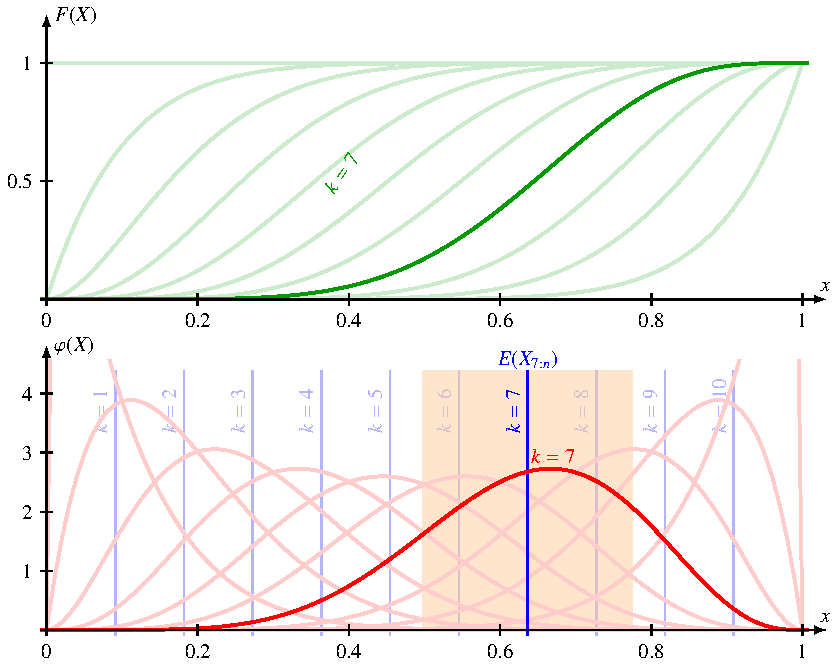
\includegraphics{chapters/040-rekursion/images/order.pdf}
\caption{Verteilungsfunktion und Wahrscheinlichkeitsdichte der
Ordnungsstatistiken $X_{k:n}$ einer gleichverteilung Zuvallsvariable
mit $n=10$.
\label{buch:rekursion:ordnung:fig:order}}
\end{figure}

%
% Die Beta-Funktion
%
\subsection{Die Beta-Verteilung
\label{buch:rekursion:subsection:beta-verteilung}}
Die Wahrscheinlichkeitsdichte, die im
Abschnitt~\ref{buch:rekursion:ordnung:section:ordnungsstatistik}
gefunden worden ist, ist nicht nur für ganzzahlige Exponenten
definiert.

\begin{figure}
\centering
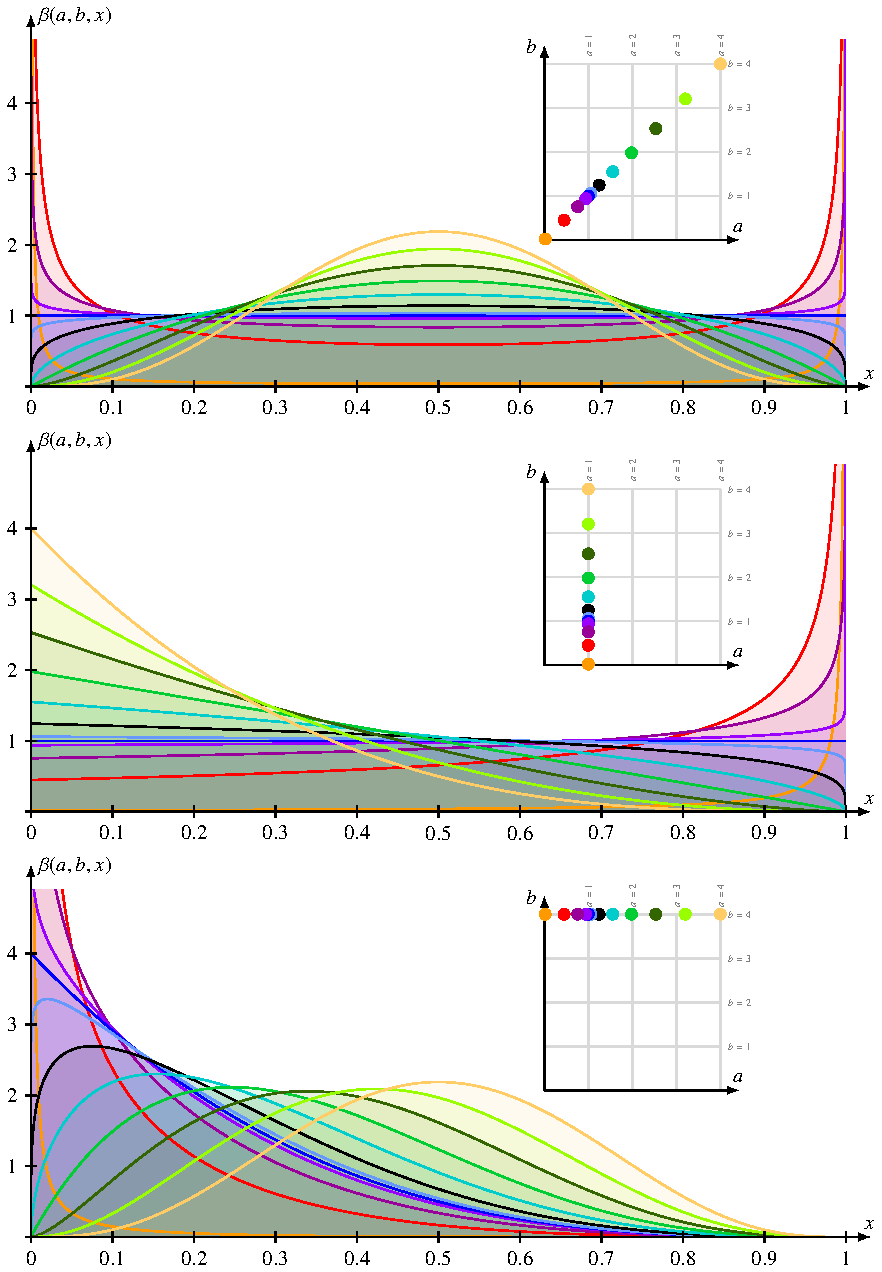
\includegraphics[width=0.92\textwidth]{chapters/040-rekursion/images/beta.pdf}
\caption{Wahrscheinlichkeitsdichte der Beta-Verteilung
$\beta(a,b,x)$
für verschiedene Werte der Parameter $a$ und $b$.
Die Werte des Parameters für einen Graphen einer Beta-Verteilung
sind im kleinen Quadrat rechts im Graphen
als Punkt mit der gleichen Farbe dargestellt.
\label{buch:rekursion:ordnung:fig:betaverteilungn}}
\end{figure}

\begin{definition}
Die Beta-Verteilung ist die Verteilung mit der Wahrscheinlichkeitsdichte
\[
\beta_{a,b}(x)
=
\begin{cases}
\displaystyle
\frac{1}{B(a,b)}
x^{a-1}(1-x)^{b-1}&\qquad 0\le x \le 1\\
0&\qquad\text{sonst.}
\end{cases}
\]
\end{definition}

Die Beta-Funktion ist also die Normierungskonstante der Beta-Verteilung.
Die wichtigsten Kennzahlen der Beta-Verteilung wie Erwartungswert und
Varianz lassen sich alle ebenfalls als Werte der Beta-Funktion ausdrücken.

\subsubsection{Erwartungswert}
Mit der Wahrscheinlichkeitsdichte kann man jetzt auch den Erwartungswerte
der $k$-ten Ordnungsstatistik bestimmen.
Die Rechnung ergibt:
\begin{align*}
E(X_{k:n})
&=
\int_0^1 x\cdot k\binom{n}{k} x^{k-1}(1-x)^{n-k}\,dx
=
k
\binom{n}{k}
\int_0^1
x^{k}(1-x)^{n-k}\,dx.
\intertext{Dies ist das Beta-Integral}
&=
k\binom{n}{k}
B(k+1,n-k+1)
\intertext{welches man durch Gamma-Funktionen bzw.~durch Fakultäten wie in}
&=
k\frac{n!}{k!(n-k)!}
\frac{\Gamma(k+1)\Gamma(n-k+1)}{n+2}
=
k\frac{n!}{k!(n-k)!}
\frac{k!(n-k)!}{(n+1)!}
=
\frac{k}{n+1}
\end{align*}
ausdrücken kann.
Die Erwartungswerte haben also regelmässige Abstände, sie sind in
Abbildung~\ref{buch:rekursion:ordnung:fig:order} als blaue vertikale Linien eingezeichnet.

Für die Beta-Verteilung lässt sich die Rechnung noch allgemeiner 
durchführen.
Der Erwartungswert einer $\beta_{a,b}$-verteilten Zufallsvariablen $X$
ist
\begin{align*}
E(X)
&=
\int_0^1 x \beta_{a,b}(x)\,dx
=
\frac{1}{B(a,b)}
\int_0^1 x\cdot x^{a-1}(1-x)^{b-1}\,dx
=
\frac{B(a+1,b)}{B(a,b)}
=
\frac{a}{a+b}.
\end{align*}
Durch Einsetzen von $a=k+1$ und $b=n-k+1$ lassen sich die für die
Ordnungsstatistik berechneten Werte wiederfinden.

\subsubsection{Varianz}
Auch die Varianz lässt sich einfach berechnen, dazu muss zunächst
der Erwartungswert von $X_{k:n}^2$ bestimmt werden.
Er ist
\begin{align*}
E(X_{k:n}^2)
&=
\int_0^1 x^2\cdot k\binom{n}{k} x^{k-1}(1-x)^{n-k}\,dx
=
k
\binom{n}{k}
\int_0^1
x^{k+1}(1-x)^{n-k}\,dx.
\intertext{Auch dies ist ein Beta-Integral, nämlich}
&=
k\binom{n}{k}
B(k+2,n-k+1)
=
k\frac{n!}{k!(n-k)!}
\frac{(k+1)!(n-k)!}{(n+2)!}
=
\frac{k(k+1)}{(n+1)(n+2)}.
\end{align*}
Die Varianz wird damit
\begin{align}
\operatorname{var}(X_{k:n})
&=
E(X_{k:n}^2) - E(X_{k:n})^2
\notag
\\
&
=
\frac{k(k+1)}{(n+1)(n+2)}-\frac{k^2}{(n+1)^2}
=
\frac{k(k+1)(n+1)-k^2(n+2)}{(n+1)^2(n+2)}
=
\frac{k(n-k+1)}{(n+1)^2(n+2)}.
\label{buch:rekursion:ordnung:eqn:ordnungsstatistik:varianz}
\end{align}
In Abbildung~\ref{buch:rekursion:ordnung:fig:order} ist die Varianz der
Ordnungsstatistik $X_{k:n}$ für $k=7$ und $n=10$ als oranges
Rechteck dargestellt.

Auch die Varianz kann ganz allgemein für die Beta-Verteilung
bestimmt werden.
Dazu berechnen wir zunächst
\begin{align*}
E(X^2)
&=
\frac{1}{B(a,b)}
\int_0^1
x^2\cdot x^{a-1}(1-y)^{b-1}\,dx
=
\frac{B(a+2,b)}{B(a,b)}.
\end{align*}
Daraus folgt dann 
\[
\operatorname{var}(X)
=
E(X^2)-E(X)^2
=
\frac{B(a+2,b)B(a,b)-B(a+1,b)^2}{B(a,b)^2}.
\]

Die Formel~\eqref{buch:rekursion:ordnung:eqn:ordnungsstatistik:varianz}
besagt auch, dass die Varianz der proportional ist zu $k((n+1)-k)$.
Dieser Ausdruck ist am grössten für $k=(n+1)/2$, die Varianz ist
also grösser für die ``mittleren'' Ordnungstatistiken als für die
extremen $X_{1:n}=\operatorname{min}(X_1,\dots,X_n)$ und
$X_{n:n}=\operatorname{max}(X_1,\dots,X_n)$.



\subsection{Weitere Eigenschaften der Gamma-Funktion}
Die nahe Verwandtschaft der Gamma- mit der Beta-Funktion ermöglicht
nun, weitere Eigenschaften der Gamma-Funktion mit Hilfe der Beta-Funktion
herzuleiten.

\subsubsection{Nochmals der Wert von $\Gamma(\frac12)$?}
Der Wert von $\Gamma(\frac12)=\sqrt{\pi}$ wurde bereits in
\eqref{buch:rekursion:gamma:wert12}
direkt mit Hilfe der Integraldefinition berechnet.
Hier wird eine alternative Berechnungsmöglichkeit mit Hilfe der
Beta-Funktion vorgestellt.

Als Anwendung der Formel~\eqref{buch:rekursion:gamma:betagamma}
untersuchen wir den Fall $y=1-x$.
In diesem Fall wird der Nenner zu $\Gamma(x+1-x)=\Gamma(1)=1$ und damit
\begin{equation}
\Gamma(x)\Gamma(1-x)
=
B(x,1-x) 
=
\int_0^1 t^{x-1}(1-t)^{-x}\,dt.
\label{buch:rekursion:gamma:spiegelung-betaintegral}
\end{equation}
Sofern man in der Lage ist, das Integral auf der rechten Seite von
\eqref{buch:rekursion:gamma:spiegelung-betaintegral} auszuwerten,
kann man eine einfache Beziehung zwischen zwei Werten der Gamma-Funktion
an Stellen, die durch eine Spiegelung an der Geraden
$\operatorname{Re}x=\frac12$ auseinander hervorgehen.
Für $x=\frac12$ wird der Ausdruck besonders einfach:
\[
\Gamma({\textstyle\frac12})^2
=
\int_0^1 t^{-\frac12}(1-t)^{-\frac12}\,dt
=
\int_0^1 \frac{1}{\sqrt{t(1-t)\mathstrut}}\,dt.
\]
Mit der Substition $t=\sin^2 s$ wird daraus
\[
\int_0^{\frac{\pi}2}
\frac{1}{
\sqrt{\sin^2s(1-\sin^2s)}
}
2\sin s\cos s
\,ds
=
2
\int_0^{\frac{\pi}2}
\,ds
=
\pi,
\]
wobei wir $dt = 2\sin s\cos s\,ds$ verwendet haben.
Somit folgt
\begin{equation}
\Gamma({\textstyle\frac12})^2 = \pi
\qquad\Rightarrow\qquad
\Gamma({\textstyle\frac12}) = \sqrt{\pi}.
\label{buch:rekursion:gamma:gamma12}
\end{equation}
Matt Parker hat auf seinem Youtube-Kanal {\em Stand-up Maths} dieses Resultat
sogar zum Titel eines Videos\footnote{\url{https://youtu.be/dGnIJFzkLI4}}
gemacht:
{\em What is the factorial of $-\nicefrac{1}{2}$?}
Die Antwort ist natürlich nur möglich, indem man
$(-\frac12)!$ als Wert
\[
(-{\textstyle\frac12})!
=
\Gamma(-{\textstyle\frac12}+1)
=
\Gamma({\textstyle\frac12})
=
\sqrt{\pi}
\]
der Gamma-Funktion interpretiert.

%
% Alternative Parametrisierung
%
\subsubsection{Alternative Parametrisierungen}
Die Substitution $t=\sin^2 s$ hat im vorangegangenen Abschnitt
ermöglicht, $\Gamma(\frac12)$ zu ermitteln.
Die Substition erlaubt aber auch, das Beta-Integral in eine alternative
Form zu bringen.
Aus der Definition~\ref{buch:rekursion:gamma:def:beta-funktion}
wird damit
\begin{align*}
B(x,y)
&=
\int_0^1 t^{x-1} (1-t)^{y-1}\,dt
\\
&=
2
\int_0^{\frac{\pi}2} \sin^{2(x-1)} s\cdot (1-\sin^2 s)^{y-1}
\cdot \sin s\cos s\,ds
\\
&=
2
\int_0^{\frac{\pi}2} \sin^{2x-1}s \cos^{2y-1} s\,ds.
\intertext{Unter Verwendung der Formel~\eqref{buch:rekursion:gamma:betagamma},
die die Beta-Funktion durch Gamma-Funktionen auszudrücken erlaubt, findet
man die Formel}
\int_0^{\frac{\pi}2} \sin^{2x-1}s \cos^{2y-1} s\,ds
&=
\frac{\Gamma(x)\Gamma(y)}{2\Gamma(x+y)}
\end{align*}
für ein bestimmtes Integral von Potenzen von Sinus- und Kosinus-Funktionen.

Die alternative Substitution $t = s/(s+1)$ verwandelt das Beta-Integral
$B(x,y)$ in ein Integral über die positive Halbachse ab:
\begin{align}
B(x,y)
&=
\int_0^1 t^{x-1}(1-t)^{y-1}\,dt
\notag
\\
&=
\int_0^\infty
\frac{s^{x-1}}{(s+1)^{x-1}}
\frac{1}{(s+1)^{y-1}}
\frac{ds}{(s+1)^2}
\notag
\\
&=
\int_0^\infty
\frac{s^{x-1}}{(s+1)^{x+y}}\,ds,
\label{buch:rekursion:gamma:beta:sinf}
\end{align}
wobei wir
\[
\frac{dt}{ds}
=
\frac{d}{ds}
\frac{s}{s+1}
=
\frac{(s+1)-s}{(s+1)^2}
=
\frac{1}{(s+1)^2}
\]
verwendet haben.
Diese Darstellung des Beta-Integrals wird später
in Satz~\ref{buch:funktionentheorie:satz:spiegelungsformel}
dazu verwendet, die Spiegelungsformel für die Gamma-Funktion
\index{Gamma-Funktion!Spiegelungsformel}%
\index{Spiegelungsformel der Gamma-Funktion}%
herzuleiten.

Eine weitere mögliche Parametrisierung verwendet $t = (1+s)/2$
mit $dt=\frac12 ds$.
Damit wird das Beta-Integral
\begin{equation}
B(x,y)
=
\int_0^1 t^{x-1}(1-t)^{y-1}\,dt
=
\frac12
\int_{-1}^1
\biggl(\frac{1+s}2\biggr)^{x-1}
\biggl(\frac{1-s}2\biggr)^{y-1}
\,ds
=
2^{1-x-y}
\int_{-1}^1
(1+s)^{x-1}(1-s)^{y-1}
\,ds.
\label{buch:rekursion:gamma:beta:symm}
\end{equation}

%
%
%
\subsubsection{Die Verdoppelungsformel von Legendre}
Die trigonometrische Substitution kann dazu verwendet werden, die
Legendresche Verdoppelungsformel für die Gamma-Funktion herzuleiten.

\begin{satz}[Legendre]
\index{Satz!Verdoppelungsformel@Verdoppelungsformel für $\Gamma(x)$}%
\[
\Gamma(x)\Gamma(x+{\textstyle\frac12})
=
2^{1-2x}\sqrt{\pi}
\Gamma(2x)
\]
\index{Verdoppelungsformel}%
\index{Gamma-Funktion!Verdoppelungsformel von Legendre}%
\end{satz}

\begin{proof}[Beweis]
Der Wert $\Gamma(2x)$ entsteht, wenn man $B(x,x)$ mit Hilfe der
Gamma-Funktion als
\[
B(x,x)
=
\frac{\Gamma(x)^2}{\Gamma(2x)}
\]
schreibt.
Das Ziel ist, $B(x,x)$ auf einem alternativen Weg zu berechnen.

Mit Hilfe von \eqref{buch:rekursion:gamma:beta:symm}
kann man das Beta-Integral zu
\begin{align*}
B(x,x)
&=
2^{1-2x}
\int_{-1}^1
(1+s)^{x-1}(1-s)^{x-1}
\,ds
=
2^{1-2x}
\int_{-1}^1(1-s^2)^{x-1}\,ds
\end{align*}
vereinfachen.
Der Integrand ist gerade, es folgt
\[
B(x,x)
=
2^{1-2x}
\cdot 2
\int_0^1(1-s^2)^{x-1}\,ds.
\]
Das Integral kann mit der Substitution $s^2=t$ wieder in die Form
eines Beta-Integrals gebracht werden:
\begin{align*}
2\int_0^1(1-s^2)^{x-1}\,ds
&=
\int_0^1 (1-t)^{x-1} \,\frac{dt}{\sqrt{t}}
=
\int_0^1 t^{\frac12-1}(1-t)^{x-1}\,dt
=
B({\textstyle\frac12},x).
\end{align*}
In der Substitution haben wir $2s\,ds = dt$ oder $2\,ds = dt/\sqrt{t}$
verwendet.
Das letzte Beta-Integral kann man nun wieder mit Gamma-Funktionen
schreiben, nämlich als
\[
B({\textstyle\frac12},x)
=
\frac{\Gamma({\textstyle\frac12})\Gamma(x)}{\Gamma(x+{\textstyle\frac12})}.
\]
Setzt man alles zusammen, erhält man jetzt
\begin{align*}
\frac{\Gamma(x)^2}{\Gamma(2x)}
&=
\frac1{2^{2x-1}}
\frac{\Gamma({\textstyle\frac12})\Gamma(x)}{\Gamma(x+{\textstyle\frac12})}
\\
\Rightarrow\qquad
\Gamma(x)\Gamma(x+{\textstyle\frac12})
&=
2^{1-2x}
\Gamma({\textstyle\frac12})\Gamma(2x)
=
2^{1-2x}\sqrt{\pi}\Gamma(2x),
\end{align*}
wobei wir den bekannten Wert $\Gamma(\frac12)=\sqrt{\pi}$ verwendet haben.
\end{proof}

Setzt man $x=\frac12$ in die Verdoppelungsformel ein, erhält man
\[
\Gamma({\textstyle\frac12})\Gamma(1) = 2^{1-2\frac12}\sqrt{\pi}\Gamma(1)
\qquad\Rightarrow\qquad
\Gamma({\textstyle\frac12}) = \sqrt{\pi},
\]
in Übereinstimmung mit dem aus \eqref{buch:rekursion:gamma:gamma12}
bereits bekannten Wert.

